\documentclass[tikz,border=4pt]{standalone}
\usepackage{tikz}
\usepackage{amsmath}
\usetikzlibrary{calc,arrows.meta,positioning,shapes.geometric,patterns}

\begin{document}
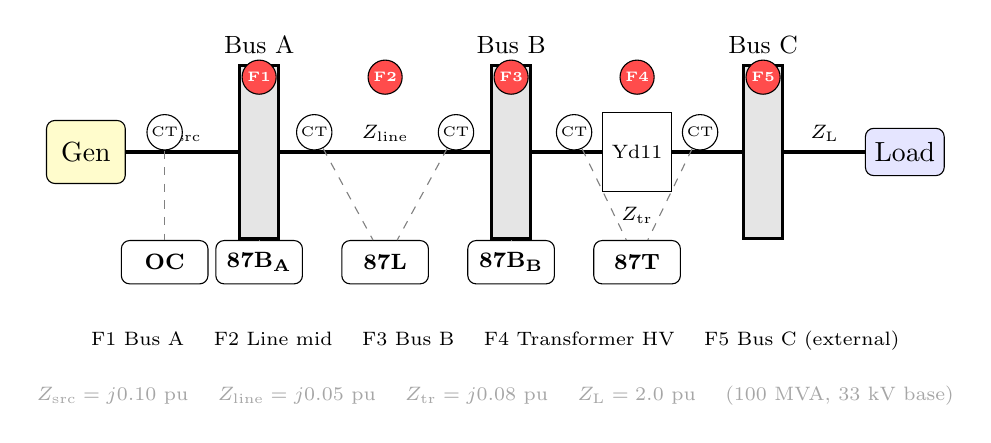
\begin{tikzpicture}[
    bus/.style={draw,fill=gray!20,minimum width=0.5cm,minimum height=2.2cm,
                inner sep=0pt,line width=1.2pt},
    relay/.style={draw,fill=white,rounded corners=3pt,font=\footnotesize\bfseries,
                  minimum width=1.1cm,minimum height=0.55cm,inner sep=2pt},
    genbox/.style={draw,fill=yellow!20,minimum width=1.0cm,minimum height=0.8cm,
                   rounded corners=3pt},
    loadbox/.style={draw,fill=blue!10,minimum width=0.8cm,minimum height=0.6cm,
                    rounded corners=3pt},
    zone/.style={draw,dashed,rounded corners=4pt,line width=0.8pt},
    annotation/.style={font=\scriptsize,text=gray!70},
    ct/.style={draw,circle,fill=white,inner sep=1pt,font=\tiny,minimum size=0.32cm},
]

% ---- x positions ---------------------------------------------------------
\def\xGen{0}
\def\xBusA{2.2}
\def\xBusB{5.4}
\def\xBusC{8.6}
\def\xLoad{10.4}
\def\yBus{0}

% ---- Buses ---------------------------------------------------------------
\node[bus,label={[font=\small]above:Bus~A}] (busA) at (\xBusA,\yBus) {};
\node[bus,label={[font=\small]above:Bus~B}] (busB) at (\xBusB,\yBus) {};
\node[bus,label={[font=\small]above:Bus~C}] (busC) at (\xBusC,\yBus) {};

% ---- Generator -----------------------------------------------------------
\node[genbox] (gen) at (\xGen,\yBus) {Gen};
\draw[line width=1.2pt] (gen.east) -- (busA.west)
    node[midway,above,font=\scriptsize] {$Z_{\rm src}$};

% ---- Line A→B -----------------------------------------------------------
\draw[line width=1.2pt] (busA.east) -- (busB.west)
    node[midway,above,font=\scriptsize] {$Z_{\rm line}$};

% ---- Transformer B→C ----------------------------------------------------
\node[draw,fill=white,minimum width=0.5cm,minimum height=1.0cm,
      label={[font=\scriptsize,yshift=-2pt]south:$Z_{\rm tr}$}]
      (tr) at (7.0,\yBus) {$\scriptstyle \text{Yd11}$};
\draw[line width=1.2pt] (busB.east) -- (tr.west);
\draw[line width=1.2pt] (tr.east) -- (busC.west);

% ---- Load ---------------------------------------------------------------
\node[loadbox] (load) at (\xLoad,\yBus) {Load};
\draw[line width=1.2pt] (busC.east) -- (load.west)
    node[midway,above,font=\scriptsize] {$Z_{\rm L}$};

% ---- CTs (small circles on conductors) ----------------------------------
% OC: between Gen and Bus_A
\node[ct] (ct_oc) at (1.0,0.25) {\tiny CT};
% 87L near/far: on line
\node[ct] (ct_Ln) at (2.9,0.25) {\tiny CT};
\node[ct] (ct_Lf) at (4.7,0.25) {\tiny CT};
% 87T HV/LV: on transformer
\node[ct] (ct_TH) at (6.2,0.25) {\tiny CT};
\node[ct] (ct_TX) at (7.8,0.25) {\tiny CT};

% ---- Relay labels --------------------------------------------------------
\node[relay] (rOC)  at (1.0,-1.4)  {OC};
\node[relay] (rBA)  at (2.2,-1.4)  {87B\textsubscript{A}};
\node[relay] (rL)   at (3.8,-1.4)  {87L};
\node[relay] (rBB)  at (5.4,-1.4)  {87B\textsubscript{B}};
\node[relay] (rT)   at (7.0,-1.4)  {87T};

\draw[dashed,gray] (ct_oc) -- (rOC);
\draw[dashed,gray] (busA)  -- (rBA);
\draw[dashed,gray] (ct_Ln) -- (rL);  \draw[dashed,gray] (ct_Lf) -- (rL);
\draw[dashed,gray] (busB)  -- (rBB);
\draw[dashed,gray] (ct_TH) -- (rT);  \draw[dashed,gray] (ct_TX) -- (rT);

% ---- Fault location markers (explicit x positions) ---------------------
\foreach \x/\lbl in {2.2/F1, 3.8/F2, 5.4/F3, 7.0/F4, 8.6/F5}
{
    \node[draw,fill=red!70,circle,inner sep=1.2pt,font=\tiny\bfseries,
          text=white] at (\x,0.95) {\lbl};
}

% ---- Fault key ----------------------------------------------------------
\node[font=\scriptsize,align=left] at (5.2,-2.4) {%
    F1 Bus~A \quad F2 Line mid \quad F3 Bus~B \quad
    F4 Transformer HV \quad F5 Bus~C (external)};

% ---- Network parameters -------------------------------------------------
\node[annotation,align=left] at (5.2,-3.1) {%
    $Z_{\rm src}=j0.10$~pu \quad $Z_{\rm line}=j0.05$~pu \quad
    $Z_{\rm tr}=j0.08$~pu \quad $Z_{\rm L}=2.0$~pu
    \quad (100~MVA, 33~kV base)};

\end{tikzpicture}
\end{document}
